\documentclass[12pt]{beamer}

\usepackage[magyar]{babel}
\usepackage[utf8]{inputenc}
\usepackage{graphicx}
\usepackage{tikz}

\hypersetup{pdfstartview={Fit}}

\usetheme{Warsaw}
\usecolortheme{whale}

\title[Ülésszervezést és jk.-írást támogató kr. készítése\hspace{4em}\insertframenumber/\inserttotalframenumber]{Ülésszervezést és jegyzőkönyv-írást támogató keretrendszer készítése}
\author{Fási Gábor}
\institute{Témavezető: Dulai Tibor}
\date{}

\begin{document}

\frame{\titlepage}

\begin{frame}
    \frametitle{Áttekintés}
    \Large
    \begin{enumerate}
        \item Feladat összefoglalása
        \item Választott technológia
        \item A rendszer moduljai
        \item Kritikus részek
        \item A megoldás értékelése
    \end{enumerate}
\end{frame}

\begin{frame}
    \frametitle{Feladat összefoglalása}
    
    \Large
    \begin{itemize}
	    \item Böngészőben működő
	    \item Ülések hirdetése
	    \item Ülések jegyzőkönyveinek készítése
	    \item Jegyzőkönyvek publikálása
	    \item Elsődlegesen a Hallgatói Önkormányzatnak, de fontos a testreszabhatóság
    \end{itemize}
\end{frame}

%valasztott technologia
\begin{frame}
    \frametitle{Választott technológia}

    \Large
    Hangsúly a nyílt, ingyenes rendszereken.
    
    \begin{itemize}
        \item PHP alapon
        \item Symfony2 keretrendszerrel
        \item Bootstrap kinézettel
    \end{itemize}
~\\~\\~\\~
    ~~~~~~~~~~~~~~~
\includegraphics[center,width=0.3\textwidth,center]{logok.png}
\end{frame}

\begin{frame}
    \frametitle{Választott technológia}
    \framesubtitle{Symfony2}
    
    \large
    \begin{itemize}
        \item Az egyik első php5.3 alapú nagy keretrendszer
        \item általános célú\\
            \small{Yahoo!, Dailymotion}
        \large            
        \item 2.0 megjelenése 2011-ben, aktuális: 2.3.0
        \item Doctrine ORM-mel együttműködés
        \item Nagyon élénk közösség
    \end{itemize}
\end{frame}

%modulok
\begin{frame}
    \frametitle{A rendszer moduljai}
    \Large
    
    Három modul:
    
    \begin{enumerate}
        \item Felhasználókezelés
        \item Ülések kezelése
        \item Jegyzőkönyvek készítése és kezelése
    \end{enumerate}
\end{frame}

%felhasznalo modul
\begin{frame}
    \frametitle{A rendszer moduljai}
    \framesubtitle{Felhasználókezelés}
    
    \begin{itemize}
        \item Authentikáció, authorizáció
        \item Felhasználók létrehozása, szerkesztése
        \item Jogosultságok kiosztása
    \end{itemize}
    
    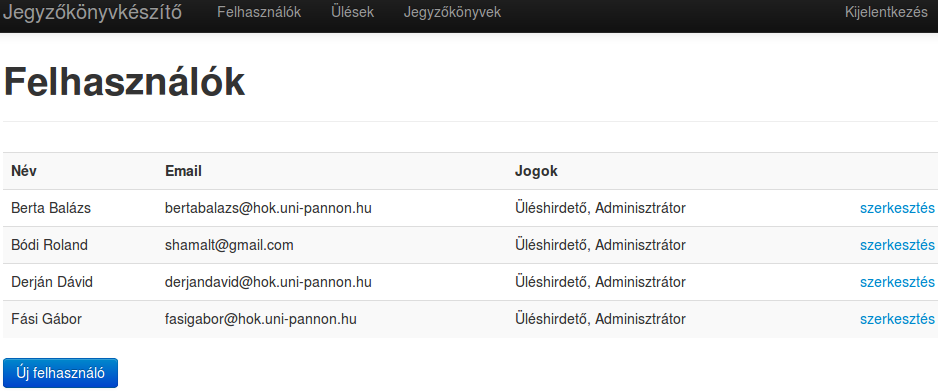
\includegraphics[width=\textwidth,center]{felhasznalolista.png}   
\end{frame}

%ules modul
\begin{frame}
    \frametitle{A rendszer moduljai}
    \framesubtitle{Ülések kezelése}
    
    \begin{itemize}
        \item Ülések létrehozása, szerkesztése
        \item Meghívottak kezelése
        \item Dokumentumok feltöltése
    \end{itemize}
    
    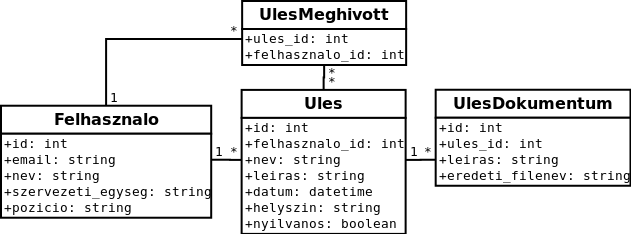
\includegraphics[width=\textwidth,center]{ules_db.png}
\end{frame}

%jegyzokonyv modul
\begin{frame}
    \frametitle{A rendszer moduljai}
    \framesubtitle{Jegyzőkönyvek készítése és kezelése}
    
    \Large
    \begin{itemize}
        \item Üléshez párosítható
        \item Egyszerű és kényelmes szerkesztés
        \item Hitelesítés
        \item PDF exportálás
    \end{itemize}
\end{frame}

\begin{frame}
    \frametitle{A rendszer moduljai}
    \framesubtitle{Jegyzőkönyvek készítése és kezelése -- adatbázis}
    
    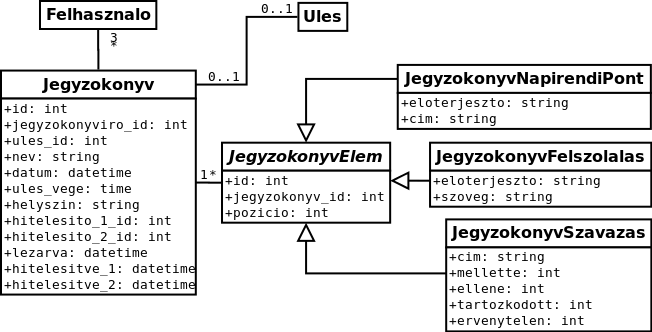
\includegraphics[width=\textwidth,center]{jegyzokonyv_db.png}
\end{frame}

\begin{frame}
    \frametitle{A rendszer moduljai}
    \framesubtitle{Jegyzőkönyvek készítése és kezelése -- szerkesztőfelület}
    
    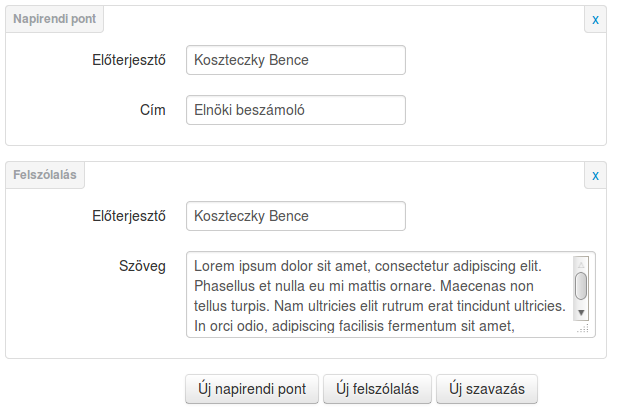
\includegraphics[width=\textwidth,center]{jegyzokonyv-szerkesztes.png}
\end{frame}

%kritikus reszek
\begin{frame}
    \frametitle{Kritikus részek}
    
    \Large
    \begin{enumerate}
        \item Jegyzőkönyv mentése
        \item PDF exportálás
        \item Google Naptár integráció
    \end{enumerate}
\end{frame}

\begin{frame}
    \frametitle{Kritikus részek}
    \framesubtitle{Jegyzőkönyv mentése}

    \large    
    \begin{itemize}
        \item Klienstől kapott és adatbázisban levő adatok összefésülése
        \item A rendszer legbonyolultabb algoritmusa
        \item Új létrehozásakor és létező szerkesztésekor
    \end{itemize}
\end{frame}

\begin{frame}
    \frametitle{Kritikus részek}
    \framesubtitle{PDF exportálás}
    
    \large
    Jegyzőkönyv, határozatok tára
    
    \begin{itemize}
        \item mPDF könyvtár
        \item HTML alapú\\
            \small a Symfony2 View rétegére építve
        \large
        \item Könnyen testreszabható
    \end{itemize}

    \begin{center}
        
\includegraphics[center,width=0.8\textwidth,center]{jegyzokonyv-fejlec.png}
    \end{center}
\end{frame}

\begin{frame}
    \frametitle{Kritikus részek}
    \framesubtitle{Google Naptár}
    \large
    
    Hirdetett ülésekről naptárbejegyzés létehozása.
    
    \begin{itemize}
        \item Jól dokumentált API
        \item Több haszálható klienskönyvtár\\
        \begin{itemize}
        	\item Hivatalos, általános célú
        	\item Zend Framework, általános, naptár komponens
        \end{itemize}            
    \end{itemize}
\end{frame}

%allapot
\begin{frame}
    \frametitle{A megoldás értékelése}
    
    \Large
    \begin{itemize}
        \item Kész rendszer
        \item A kiírt feladatot megvalósítja
        \item Április óta használatban
        \item Felhasználói visszajelzések is beépítve
    \end{itemize}
\end{frame}

\end{document}
